\chapter{Theoretical Background}\label{chap:theory}

\section{Plasma Generation and Composition}

\subsection{Cathode Spot Plasma Generation}

Cathodic‐arc plasmas form at microscopic emission centers, known as cathode spots, on an otherwise cold metal electrode under vacuum. Spot ignition occurs when the local cathode surface, through breakdown of adsorbates or field-enhanced thermionic emission, undergoes a rapid, explosive release of electrons and vaporized metal. During a single spot pulse, a few nanograms of the cathode material rapidly heat up, vaporize, and ionize, producing a dense, quasineutral plasma plume composed mostly of metal ions and electrons. The peak spot current densities reach \(10^{10}\)–\(10^{12}\)\,A\,m\(^{-2}\), far above steady-state thermionic or field emission limits. These microexplosions, termed ectons (explosive electron emission centers), produce localized nanosecond-scale plasma bursts. The arc is sustained by repetitive ecton events occurring at or near the same location \cite[Chap.~3.3--3.4]{cathodic_arcs}.\\




Key Characteristics of Spot-Generated Plasma:
\begin{itemize}
    \item High degree of ionization: >90 \% of the ejected metal atoms emerge as ions, a consequence of the extreme power density in the cathode spot \cite[Chap.~3.5]{cathodic_arcs}.
    \item Multiply charged ions: the charge state distributions extend to \(Q=3\)–4 for refractory metals, such as Ti and Al, due to the high electron temperature and density in the spot plasma \cite[Chap.~3.5]{cathodic_arcs}.
    \item Transient, localized heating: the sub-µm, sub-100 ns pulse produces “atomic‐scale heating”, where the energy of individual ions is deposited in a highly localized region upon impact, influencing film growth and microstructure \cite[Chap.~3.6]{cathodic_arcs}.
\end{itemize}

\begin{figure}[h]
	\centering
	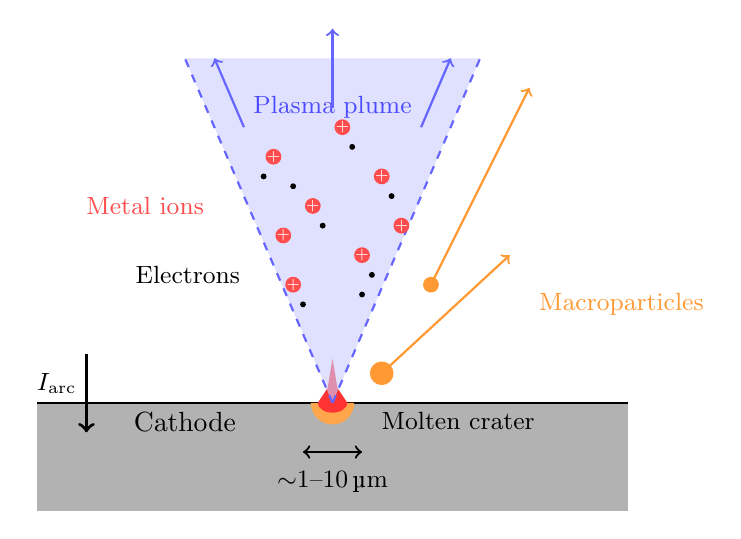
\begin{tikzpicture}[scale=1.25]
		% Cathode block
		\fill[gray!60] (-3,-1.1) rectangle (3,0);
		\draw[thick] (-3,0) -- (3,0);
		\node[below] at (-1.5,0) {Cathode};
		
		% Molten crater
		\fill[orange!70] (-0.22,0) arc (180:360:0.22) -- cycle;
		\fill[red!80] (-0.15,0) arc (180:360:0.15 and 0.1) -- (0.15,0) -- (0.05,0.15) -- (0,0.45) -- (-0.05,0.15) -- (-0.15,0) -- cycle;
		\node[below right, font=\small] at (0.4,0) {Molten crater};
		
		% Plasma plume (expanding cone)
		\fill[blue!20, opacity=0.6] (0,0) -- (-1.5,3.5) -- (1.5,3.5) -- cycle;
		\draw[blue!60, thick, dashed] (0,0) -- (-1.5,3.5);
		\draw[blue!60, thick, dashed] (0,0) -- (1.5,3.5);
		\node[blue!70, font=\small] at (0,3) {Plasma plume};
		
		% Ions (circles with + signs)
		\foreach \x/\y in {-0.4/1.2, 0.3/1.5, -0.2/2.0, 0.5/2.3, -0.6/2.5, 0.1/2.8, 0.7/1.8, -0.5/1.7} {
			\fill[red!70] (\x,\y) circle (0.08);
			\node[white, font=\tiny] at (\x,\y) {+};
		}
		\node[red!70, right, font=\small] at (-2.6,2.0) {Metal ions};
		
		% Electrons (small dots)
		\foreach \x/\y in {-0.3/1.0, 0.4/1.3, -0.1/1.8, 0.6/2.1, -0.7/2.3, 0.2/2.6, -0.4/2.2, 0.3/1.1} {
			\fill[black] (\x,\y) circle (0.03);
		}
		\node[right, font=\small] at (-2.1,1.3) {Electrons};
		
		% Macroparticle (larger droplet trajectory)
		\fill[orange!80] (0.5,0.3) circle (0.12);
		\draw[->, thick, orange!80] (0.5,0.3) -- (1.8,1.5);
		\fill[orange!80] (1,1.2) circle (0.08);
		\draw[->, thick, orange!80] (1,1.2) -- (2,3.2);
		\node[orange!80, right, font=\small] at (2.0,1.0) {Macroparticles};
		
		% Current flow arrow
		\draw[->, very thick] (-2.5,0.5) -- (-2.5,-0.3);
		\node[left, font=\small] at (-2.5,0.2) {$I_{\rm arc}$};
		
		% Spot diameter indicator
		\draw[<->, thick] (-0.3,-0.5) -- (0.3,-0.5);
		\node[below, font=\small] at (0,-0.6) {$\sim$1--10\,\textmu m};
		
		% Expansion arrows
		\draw[->, thick, blue!60] (0,3.0) -- (0,3.8);
		\draw[->, thick, blue!60] (-0.9,2.8) -- (-1.2,3.5);
		\draw[->, thick, blue!60] (0.9,2.8) -- (1.2,3.5);
		
	\end{tikzpicture}
	\caption{Schematic of cathode spot operation. The arc current $I_{\rm arc}$ concentrates at a microscopic spot (1--10\,\textmu m diameter), creating a molten crater from which a plasma plume of metal ions and electrons expands. Macroparticles (molten droplets) are ejected at oblique angles. Adapted from \cite{juttner2001}}.
	\label{fig:cathode_spot}
\end{figure}


Spot ignition and quenching occur on timescales of 10–100 ns, with each pulse ejecting a fully ionized burst of metal vapour. The sustained arc discharge thus consists of continuously overlapping microplasma pulses, producing a metal-rich, high-flux ion stream well-suited for energetic thin-film deposition.\\


\subsection{Plasma Composition and Expansion}

After generation at the cathode spots, the metal-rich plasma expands into the vacuum chamber, typically passing through a magnetic macroparticle filter that removes molten droplets while guiding ions along curved field lines. In the region near the cathode (within a few centimeters of the spot), plasma densities are on the order of \(10^{18}\) cm$^{-3}$ and electron temperatures \(T_e\approx5\ \text{–}\ 10\) eV. As the plume propagates, its density decreases according to
\begin{equation}
    n(r) = \frac{C\,I_{\rm arc}}{r^2}
\end{equation}
where \(I_{\rm arc}\) is the arc current, $r$ the distance, and $C$ a constant related to the ion‐erosion rate of the cathode material. This $\frac{1}{r^2}$ scaling assumes free expansion, but deviations can occur due to magnetic fields, collisions, or reactive gases, which may alter the plasma trajectory or cause recombination \cite[Chap.~4.3; Eq.~4.3, p.~178]{cathodic_arcs}.\\

In cathodic‐arc discharges from titanium cathodes, whether pure Ti or Ti–Al compounds, ions generally carry an average charge state \(\langle Q\rangle\approx2.1\text{–}2.2\) \cite[Chap.~4.1; App.~B.8]{cathodic_arcs}. This high degree of ionization reflects the extreme power density of the spot and follows the cohesive energy rule, which links \(\langle Q\rangle\) to the cohesive energy of the cathode material (Table B.8) \cite[App.~B.8]{cathodic_arcs}.

%Applying an external axial magnetic field at the source (the “EM-coil” configuration) can boost ⟨Q⟩ by 10–30 \% and increase total ion flux by up to an order of magnitude. Effects attributed to enhanced magnetic insulation and longer plasma spot interaction times \cite{decoupling_kalanov_2025}. In contrast, imposing a DC bias on the source raises the ions’ kinetic energy with minimal change to ⟨Q⟩ or flux, offering a route to decouple kinetic and potential-energy contributions in film-growth studies.\\


\section{Ion Energy and Flux}

\subsection{Ion Energies: Origins and Implications}
\label{section:ion_energies}
Ion energies in cathodic-arc plasmas have been extensively characterized through time-of-flight measurements. For the materials relevant to this work both exceeding the $\approx 30$\,eV threshold for subplantation when combining the kinetic and potential energy as can be seen in Table \ref{tab:ion_properties}. This enables densification and improved crystallinity in Ti–Al–N films without requiring external substrate heating \cite[Chap.~8.1--8.2]{cathodic_arcs}.\\

\begin{table}[htbp]
	\centering
	\caption{Characteristic ion properties for Ti and Al cathodic-arc plasmas in vacuum \cite[App.~B; Table~B.8]{cathodic_arcs}.}
	\label{tab:ion_properties}
	\begin{tabular}{lcccc}
		\hline
		Species & $\langle Q \rangle$ & $E_{\rm kin}$ (eV) & $E_{\rm pot}$ (eV) & $E_{\rm tot}$ (eV) \\
		\hline
		Ti$^{2+}$ & 2.1 & 59 & 21 & 80 \\
		Al$^{2+}$ & 1.7 & 28 & 24 & 52 \\
		\hline
	\end{tabular}
\end{table}


While ion energy influences film properties, this work focuses on quantifying the flux of both metal ions and reactive nitrogen species to understand their combined role in film growth. In metallic mode, the narrow energy distribution simplifies flux measurements and enables direct correlation with deposition rate. In reactive mode, collisions with N$_2$ broaden the energy distribution and generate additional species, N$^+$, N$_2^+$, and metastable N$_2$, that must be distinguished in mass spectrometer measurements \cite{bendikt2012}.\\

To isolate the effects of ion flux and reactive nitrogen, we systematically vary the N$_2$ pressure and adjust the magnetic field strength, ensuring that changes in film properties reflect controlled variations in plasma composition rather than incidental energy shifts.




\subsection{Ion Flux and Diagnostics}
\label{section:ion_flux}

The ion flux $\Gamma$ represents the number of ions arriving per unit area per unit time, expressed in ions\,cm$^{-2}$\,s$^{-1}$. In a multiply charged plasma, the total measured ion current density $J_i$ (A\,cm$^{-2}$) relates to $\Gamma$ via
\begin{equation}
	\Gamma = \frac{J_i}{e\,\langle Q \rangle},
\end{equation}
where $e$ is the elementary charge and $\langle Q \rangle$ the average ion charge state. This relationship is central to correlating time-averaged ion flux with deposited mass.\\

To compare ion fluxes across different materials and arc currents, the particle system coefficient
\begin{equation}
	k_{\rm part} = \frac{I_i}{\langle Q \rangle\,I_{\rm arc}}
\end{equation}
normalizes the measured probe current $I_i$ by the arc current $I_{\rm arc}$ and accounts for variations in $\langle Q \rangle$ \cite[Chap.~6.5]{cathodic_arcs}. This normalization is necessary because the probe measures electrical current rather than particle flux, and multiply charged ions contribute proportionally more current per particle.\\

In vacuum cathodic arcs, the burning voltage remains nearly constant at 30–35\,V for arc currents up to 1\,kA, so the plasma generation rate—and thus $\Gamma$—increases approximately linearly with $I_{\rm arc}$ \cite[Chap.~6.5]{cathodic_arcs}. External magnetic fields can increase $\Gamma$ by up to an order of magnitude by confining the plasma and prolonging ion residence time near the cathode.\\

The relationship between ion flux and film growth rate is given by
\begin{equation}
	R = \frac{m_{\rm ion}\,\Gamma\,S}{\rho_{\rm film}},
\end{equation}
where $m_{\rm ion}$ is the average ion mass, $S$ the sticking coefficient, and $\rho_{\rm film}$ the film density. The sticking coefficient $S$ represents the probability that an arriving ion incorporates into the growing film rather than being reflected or resputtered; for metal ions at moderate energies (below the resputter threshold of $\sim$100–200\,eV), $S \approx 1$ is typically assumed. For constant ion energy and a sticking coefficient equal to one, the deposition rate scales linearly with ion flux. Deviations from linearity indicate that additional processes (such as densification, resputtering, or adatom crowding) influence film growth. Unutulmazsoy et al.\ observed this linear scaling in (V,Al)N films deposited by pulsed filtered cathodic arc, with deviations emerging at high flux densities where ion-induced densification becomes significant \cite{unutulmazsoy}.\\

Experimentally, ion flux is determined from biased probe measurements operating in ion saturation mode, while charge-state and energy distributions are obtained via energy-resolved mass spectrometry. The diagnostic methods used in this work are described in Chapter~\ref{chap:methods}.
To connect the theory of ion flux and energy to experimental data, we employ two primary diagnostics:

\section{Plasma--Surface Interactions and Film Growth}
\subsection{Energetic Condensation and Subplantation}

When metal ions with sufficient energy strike the growing film, they penetrate below the surface and deposit energy through a shallow collision cascade. This subplantation process produces two key effects:

\begin{itemize}
	\item \textbf{Localized densification:} Ions with energies above approximately 20–30\,eV implant beneath the surface, occupying interstitial sites and displacing near-surface atoms through knock-on collisions. This reduces porosity and increases film density, which is particularly important for transition-metal nitride coatings such as Ti--Al--N \cite[Chap.~8.1]{cathodic_arcs}.
	
	\item \textbf{Atomic-scale heating:} The deposition of kinetic energy and release of potential energy (ionization enthalpy) generate localized, nanosecond-scale temperature spikes. These enhance adatom mobility and promote crystallite coalescence without requiring global substrate heating \cite[Chap.~8.2]{cathodic_arcs}.
\end{itemize}

As $E_{\rm kin}$ and $E_{\rm pot}$ increase, films transition from porous, amorphous structures to dense, crystalline coatings. This densification introduces compressive stresses of several GPa through atomic peening \cite[Chap.~8.1--8.4]{cathodic_arcs}. For example, TiN films grown with total ion energies of approximately 60\,eV develop a preferred cubic (111) texture and hardness exceeding 30\,GPa.\\

In cathodic-arc deposition, the ion energies are primarily determined by the cathode material and plasma expansion conditions rather than external bias. The present work therefore focuses on characterizing the correlation between ion flux $\Gamma$ (measured by a biased collector probe) and deposition rate (measured by QCM), rather than systematic variation of ion energy. The results of these measurements are presented in Chapter~\ref{chap:results}.


\subsection{Reactive vs Metallic Mode}

Cathodic-arc deposition operates in two distinct regimes. In metallic mode, the cathode surface remains uncovered and the plasma consists exclusively of metal ions, characterized by stable burning voltage and high metal ion flux. In reactive mode, a background gas such as N$_2$ adsorbs onto the cathode surface, forming a compound layer that poisons the cathode and alters both spot behaviour and plasma composition \cite[Chap.~9.2]{cathodic_arcs}.\\

When N$_2$ is introduced, a dynamic equilibrium develops between compound formation, through adsorption and reaction at the cathode surface and compound removal via explosive ecton events that eject both metal and nitride fragments \cite[Chap.~9.3]{cathodic_arcs}. The equilibrium position depends on gas pressure, arc current, and cathode composition. At low N$_2$ pressures or high power densities, type-2 (metal-rich) spots prevail, maintaining predominantly metal ion flux. At higher pressures, type-1 (poisoned) spots dominate, producing a mixed plasma of metal and nitrogen ions \cite[Chap.~9.4]{cathodic_arcs}.\\

Reactive mode affects both plasma diagnostics and film growth:
\begin{compactitem}
	\item The measured probe current includes contributions from N$^+$ and N$_2^+$ in addition to metal ions, requiring mass-resolved analysis to separate species.
	
	\item Charge exchange with N$_2$ reduces the average charge state of metal ions and introduces gas-ion species, altering the potential energy budget \cite[Chap.~9.4]{cathodic_arcs}.
	
	\item Collisions during plasma expansion reduce ion drift velocities, lowering kinetic energy before substrate impact \cite[Chap.~9.4]{cathodic_arcs}.
\end{compactitem}

In the present experimental setup, N$_2$ is introduced via a ring-manifold inlet downstream of the magnetic filter, minimizing pressure gradients and enabling reproducible reactive-mode operation. By comparing measurements in vacuum and under varying N$_2$ pressures, this work investigates how reactive mode influences $\Gamma$ and $\langle Q \rangle$, and how these parameters correlate with deposited mass and film composition.

\section{Crystal Structure and Densification}

\subsection{Structure-Zone Models}

The microstructure of thin films deposited by physical vapour deposition depends strongly on the energy and flux of incident species. Thornton's structure-zone model, originally developed for magnetron sputtering, relates film morphology to the homologous temperature $T/T_m$ (substrate temperature normalized to the melting point) and working gas pressure \cite{thornton1977}. At low $T/T_m$ and high pressures, films exhibit porous, columnar structures (Zone~1) due to limited adatom mobility. As $T/T_m$ increases, denser columnar (Zone~T) and eventually equiaxed crystalline structures (Zone~2 and Zone~3) develop.\\

Anders extended this framework to account for the energetic ion bombardment characteristic of cathodic-arc deposition \cite{anders2010szm}. In the revised model, ion energy $E^*$ (normalized to a displacement energy) replaces gas pressure as the second axis, reflecting the dominant role of ion bombardment in densification. High-energy ions can induce subplantation and atomic peening even at low substrate temperatures, enabling dense, crystalline films without external heating, which is a key advantage of cathodic-arc processes. However, excessive ion energy leads to lattice damage, defect accumulation, and eventually amorphization or resputtering, defining an optimal energy window for film growth \cite[Chap.~8.3]{cathodic_arcs}.\\

\begin{figure}[htbp]
	\centering
	\includegraphics[width=0.8\textwidth]{Figures/theory/anders_szm.png}
	\caption{Structure-zone diagram for plasma-based thin film deposition, showing film microstructure as a function of generalized temperature $T^*$ and normalized ion energy $E^*$. From Anders \cite{anders2010szm}.}
	\label{fig:anders_szm}
\end{figure}


For the Ti--Al--N system, the Anders structure-zone model predicts that the multiply charged ions typical of cathodic arcs promote Zone~T or Zone~2 microstructures even at modest substrate temperatures, provided the ion flux is sufficient to maintain a high ion-to-neutral arrival ratio.


\subsection{TiAlN Crystal Structures}

Titanium aluminium nitride (Ti$_{1-x}$Al$_x$N) coatings are widely used for wear protection and cutting tools due to their high hardness, oxidation resistance, and thermal stability. The crystal structure depends primarily on the aluminium content $x$:\\


\begin{compactitem}
	\item For $x \lesssim 0.6$ – 0.7, Ti$_{1-x}$Al$_x$N crystallizes in the metastable cubic B1 structure, where Al atoms substitute for Ti on the metal sublattice. This cubic phase exhibits hardness values of 25–35\,GPa and is the preferred structure for most industrial applications \cite{paldey2003}.
	
	\item For $x \gtrsim 0.7$, the thermodynamically stable wurtzite (B4) structure becomes dominant. The wurtzite phase has lower hardness (typically 15–20\,GPa) and is generally undesirable for hard coating applications \cite{mayrhofer2006}.
	
	\item At intermediate compositions, mixed cubic-wurtzite structures or nanocomposite arrangements may form, depending on deposition conditions.
\end{compactitem}
\vspace{12pt}


The metastable cubic phase is retained at high Al contents through kinetic limitations during low-temperature deposition. Energetic ion bombardment in cathodic-arc processes can extend the solubility limit of Al in the cubic phase by providing additional energy for atomic rearrangement without the diffusion lengths associated with thermal equilibration \cite{rachbauer2011}.\\

The cathode composition used in this work (75\,wt.\% Ti – 25\,wt.\% Al is expected to produce cubic-phase Ti$_{1-x}$Al$_x$N films under typical cathodic-arc conditions. Film structure will be verified by X-ray diffraction, with microstructure examined by scanning electron microscopy, as described in Chapter~\ref{sec:film_characterization}.

